%% go to the website http://en.wikibooks.org/wiki/LaTeX For Help 
\documentclass[11.5pt]{article}
%Math Related Packages
\usepackage{mathtools}
\usepackage{amsmath}
\usepackage{amsfonts}
\usepackage{amssymb}
\usepackage{relsize}
% Pseudocode Packages
%\usepackage{algorithm}
%\usepackage{algpseudocode}
\usepackage[colorinlistoftodos]{todonotes}
% Automata/Graph Packages
\usepackage{tikz}
\usepackage{pgf}
\usetikzlibrary{arrows,automata}
\usepackage[latin1]{inputenc}
\usetikzlibrary{automata,positioning}
%%%Formatting Options for Pages
%\usepackage[a4paper,left=2cm,right=2cm]{geometry} %Change Margins
\usepackage[colorlinks=true, allcolors=blue]{hyperref} % adds hyperlinks
\usepackage{listings}
\usepackage{multicol}
\usepackage{perpage}
\MakePerPage{footnote}
%%%Graphics Packages and Caption Tools
\usepackage{graphicx}
\usepackage{fullpage}
\newcounter{Figure} 
\setcounter{Figure}{1}
%\usepackage{slashbox}
\usepackage{ulem}
\usepackage{csvsimple}
%%%Colors Package with Custom Defined Colors
\usepackage{color}
\usepackage{colortbl}
\definecolor{codegreen}{rgb}{0,0.6,.2}
\definecolor{codegray}{rgb}{0.5,0.5,0.5}
\definecolor{codepurple}{rgb}{0.58,0,0.82}
%%Custom Functions and Commands
\newcommand\indentFour{\indent\indent\indent\indent}
\newcommand\indentThree{\indent\indent\indent}
\newcommand\indentTwo{\indent\indent}
\newcommand\tab{\ \ \ }
\newcommand\proof{\setcounter{equation}{0}\hfill\fbox{\rule{.02in}{0pt}\rule[0ex]{0pt}{.5ex}}}

%%Math Commands
\newcommand{\Lbra}{\left\langle}
\newcommand{\Rbra}{\right|}
\newcommand{\Rket}{\right\rangle}
\newcommand{\Lket}{\left|}
\newcommand{\bra}[1]{\Lbra #1 \Rbra}
\newcommand{\ket}[1]{\Lket #1 \Rket}
\newcommand{\braket}[1]{\Lbra #1 \Rket}
\newcommand{\Exists}{\ \exists \ }
\newcommand{\Forall}{\ \forall \ }
\newcommand{\abs}[1]{\left| #1 \right|}
\newcommand{\Frac}[2]{\left(\frac{#1}{#2}\right)}
\newcommand{\Mat}[1]{\left[\begin{matrix} #1 \end{matrix}\right]}
\newcommand{\vhi}{\varphi}
\newcommand{\R}{\ \mathbb{R}}
\newcommand{\C}{\ \mathbb{C}}
\newcommand{\N}{\ \mathbb{N}}
\newcommand{\Z}{\ \mathbb{Z}}
\newcommand{\I}{\ \mathbb{R/Q}}
\newcommand{\x}{\mathrm{x}}
\newcommand{\mbf}[1]{\mathbf{#1}}
\newcommand{\Dpart}[2]{\frac{\partial #1}{\partial #2}}
\DeclarePairedDelimiter{\ceil}{\lceil}{\rceil}
\newcommand{\U}{\underline}
%Numbering
\newcounter{graphics}
\newcounter{tables}
\renewcommand{\abstractname}{Abstract}

\begin{document}
\title{Deep Learning for Knowledge Graph Completion}
\author{Nick, Kevin, Cesar Bartolo-Perez, Doug\\
	{\small\textit{University of California - Davis}}
} 
\date{November 30th, 2017}
\maketitle
\rule{\textwidth}{1pt}



\begin{abstract}

\end{abstract}

\tableofcontents


\section{Introduction}
An example of citing something is \cite{KosticFuso}


I'm righting something here for testing with github.

\section{Methods}
\subsection*{Multilayer Perceptron Model (MLP)}
\subsubsection{Data Formatting}
The first thing we needed to do was format the data. Some textSome textSome textSome textSome textSome textSome textSome textSome textSome textSome textSome textSome textSome textSome textSome textSome textSome textSome textSome textSome textSome textSome textSome textSome textSome textSome textSome textSome textSome textSome textSome textSome textSome textSome textSome textSome textSome textSome textSome textSome textSome textSome textSome textSome textSome textSome textSome textSome textSome textSome textSome textSome textSome textSome textSome textSome textSome textSome textSome textSome textSome textSome textSome textSome textSome textSome textSome textSome textSome textSome textSome textSome textSome textSome text

The multiyaler perceptron (MLP) model was built using the the Stuttgart Neural Network Simulator implemented in language R (RSNNS)\cite{RSNNS}. Where we have used standard backpropagation and backpropagation with momentum methods in our simulation models.

Different  MLP architectures are built, varying number of hidden layers, nodes and iterations in order to improve the accuracy and precision of our model.

Weighted SSE by number of iterations of the training and tetsing sets in addition to ROC curves will provide the references in our model architecture selection.

writing something here too for testing with github

\section{Results}

In order to prevent overfitting in our model, we have compared our model with 100 and 50 interations (Figure ~\ref{fig:50_100_128.png}). We can notice that under 100 iterations, the trainin error drops to a weigthed SSE of almost 500. However, our testing error, start increasing after 30 itearions aproximately. From this results, we can infer that we have reached an overfitting in our model and a smaller number of iterations are enougth. In that sense, we have run our model with 50 iterations, avoiding the increase in the SSE.\par
 

\begin{figure}[h!]
  \caption{MSE at different iterations. The structure presents a single hidden layer with 128 nodes}
  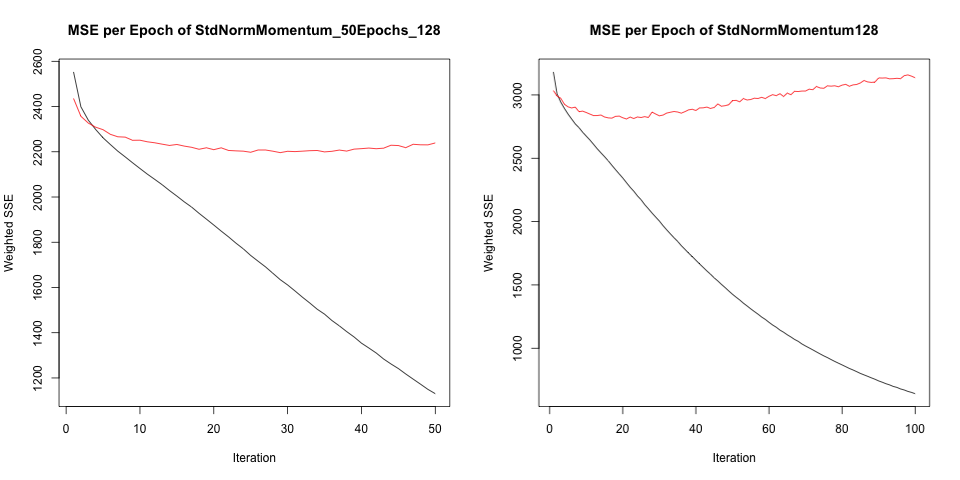
\includegraphics[width=1\textwidth]{report_mlp/50_100_128.png}

\end{figure}


In a second running of the model, we have added a new hidden layer  with different number of nodes (16,64 and 128). Before 50 iterations, adding nodes to the second hidden layer, reduce the error in our model. However, after 50 iteration, the higher number of nodes, increase rapidly the overfitting  of the model. \par 


\begin{figure}[h!]
  \caption{MSE for A NN with two hidden layers with different nodes at second hidden layer.}
  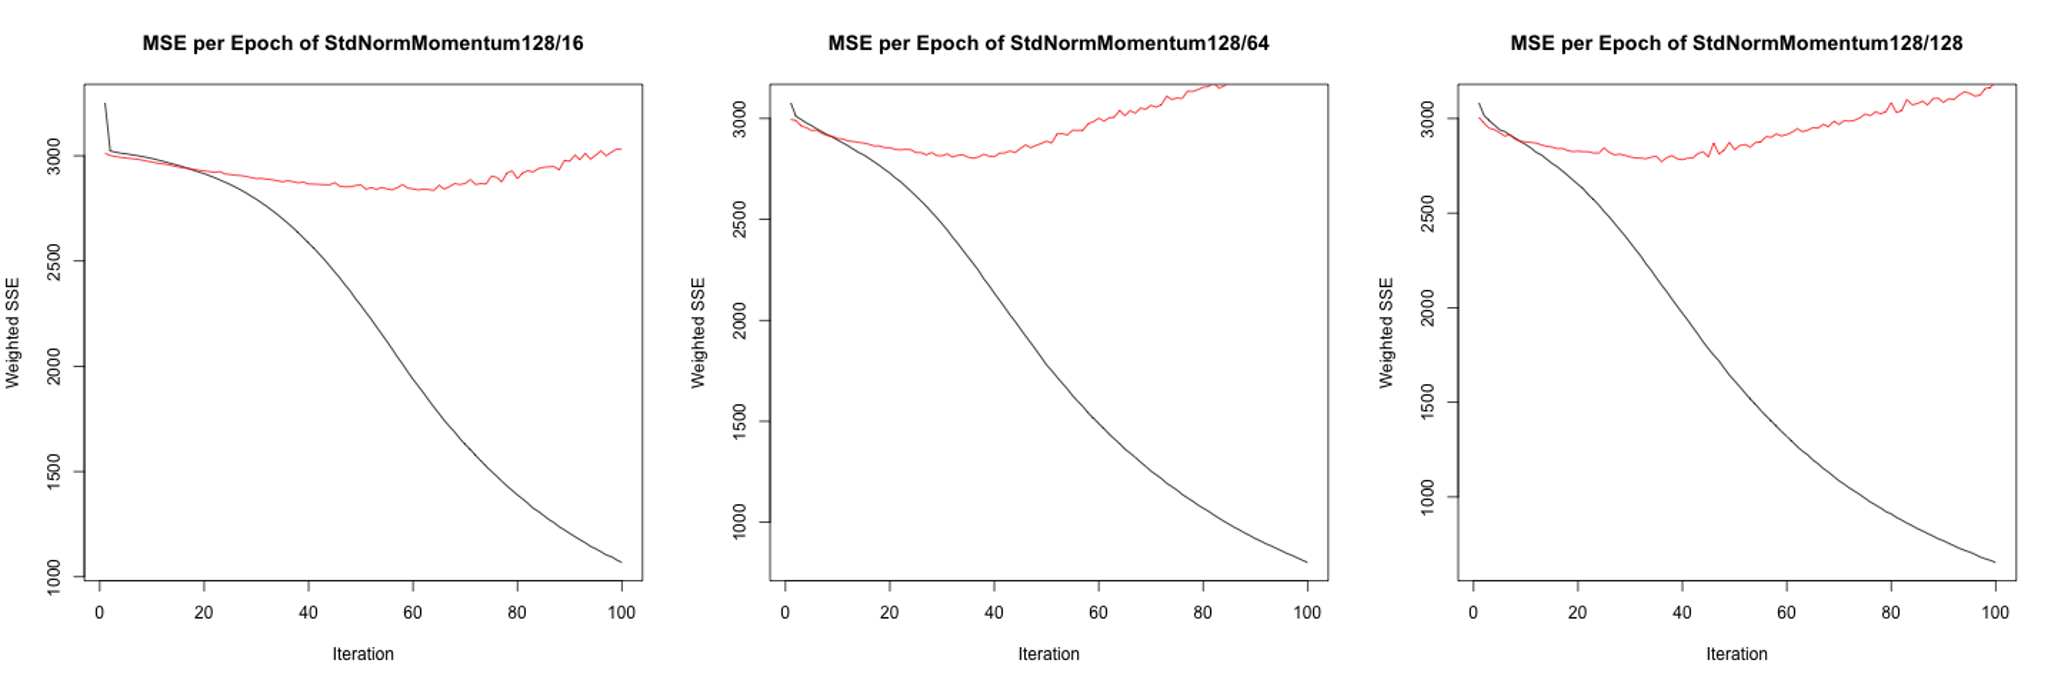
\includegraphics[width=1\textwidth]{report_mlp/128-16_64_128.png}
\end{figure}

writing something here for testing with github

In  a following set of tests, we compared different Neural Networks structures, increasing the number of hidden layers (hidden layers/nodes: 128, 128/16 and 128/128/16).  Figure ~\ref{fig:50.png} shows that for the model with three hidden layers the training error is not decreasing considerably before 40 iteration. Suddently, the SSE in this NN structure drops abruptaly. The training error, shows that the error keep increasing at that range of iterations. This beahvior, can be attributed to an overfitting in our model. \par

Ths trend described above is similar for two hidden layers. For teh case of just one hidden layer with 128 nodes, the error does not drop abruptaly for the training set but we can see an increase in the error for after 30 iterations aproximately. \par 

These results, make us suggest that only one hidden layer is enough for our MLP model, since there is not a big improvement in the reduction of error with more layers added and with the benefit of less computational resources are required.
This decision is confirmed comparing their ROC curves for each NN structure.
 








\begin{figure}[h!]
  \caption{MSE and ROC curves for different levels of hidden layers}
  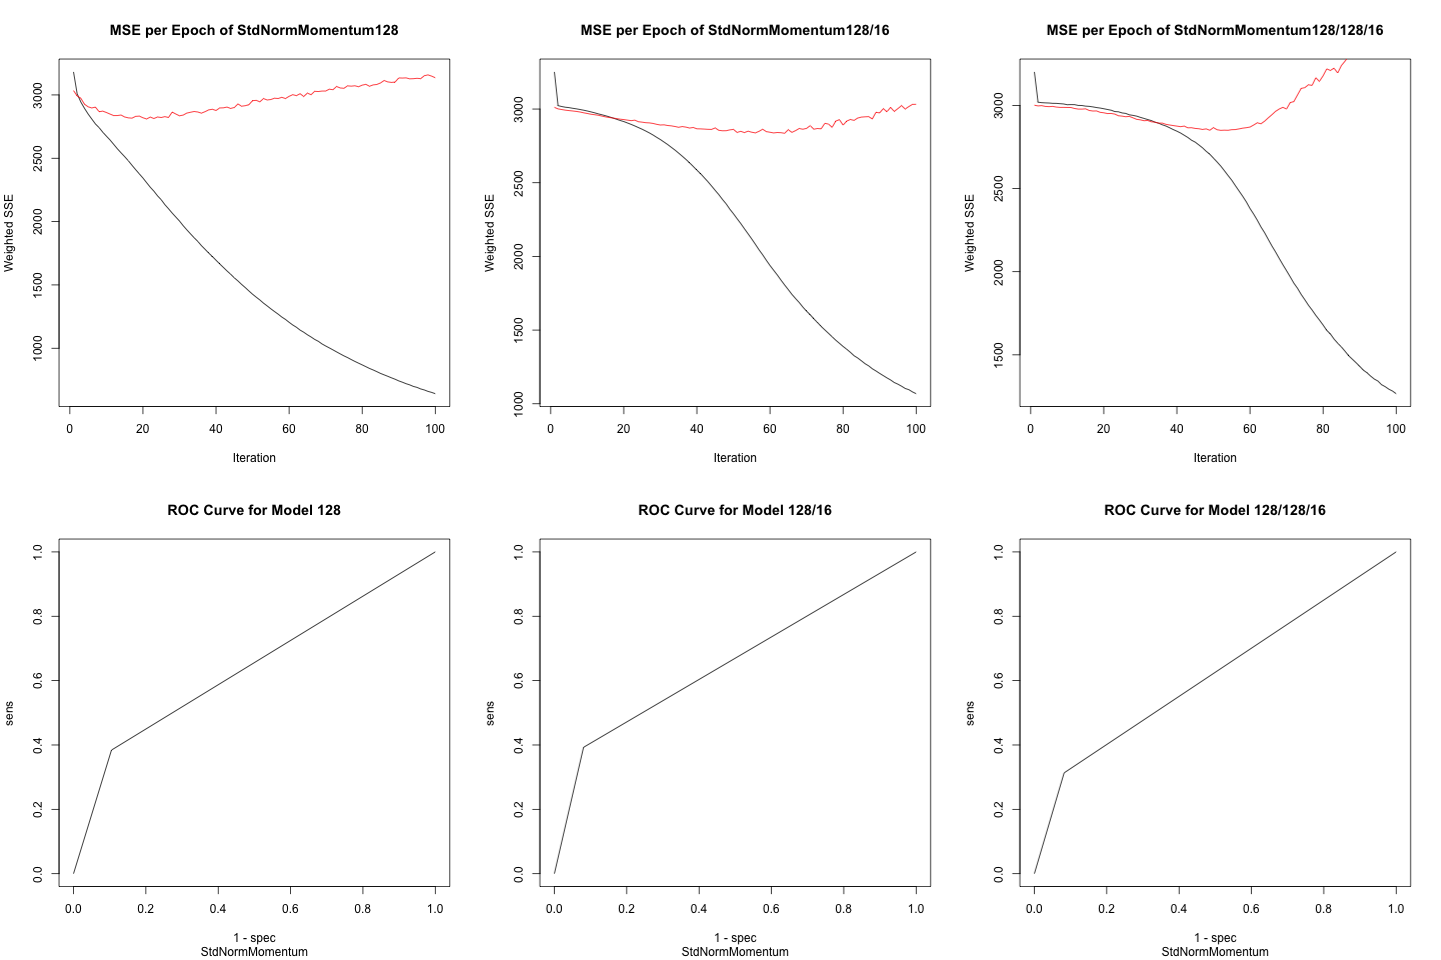
\includegraphics[width=1\textwidth]{report_mlp/different_layers_MSE_ROC.png}
\end{figure}

more tests for github



\section{Discussion}

\bibliographystyle{ieeetr}
\bibliography{bib}{}

\end{document}